% \documentclass[10pt]{beamer}
\documentclass[10pt,handout]{beamer}

% \usetheme{Pittsburgh}
\usetheme{metropolis}%great
% \usetheme{hsrm}%BEST for Presentation
%\usetheme{Hannover}%clean white best bright theme
%\usetheme{AnnArbor}%good
% \usetheme{Bergen}
% \usetheme{Berkeley}%BEST for Email
% \usetheme{Frankfurt}
% \usetheme{Warsaw}
% \usetheme{sthlm}

%\usecolortheme{owl} % dark theme
%\usecolortheme[snowy]{owl} % black on white
\usepackage{appendixnumberbeamer}
\usepackage[T1]{fontenc}
\usepackage[utf8]{inputenc}
% \usepackage{lmodern}

\usepackage{booktabs}
\usepackage[scale=2]{ccicons}
\usepackage{textcomp}

% \usepackage{pgfplots}
% \usepgfplotslibrary{dateplot}

\usepackage{xspace}
\usepackage{tabularx}
\renewcommand\tabularxcolumn[1]{m{#1}}% for vertical centering text in X column
\usepackage{adjustbox}

\newcommand{\themename}{\textbf{\textsc{metropolis}}\xspace}
\newcolumntype{Y}{>{\centering\arraybackslash}X}

\title{GPUCoin zk distributed computing future proof video protocol Ðapps platform powered by cryptocurrency Blockchain}
\subtitle{Open Source decentralized uncensorable network allowing anyone to rent their excess bandwidth \& GPU compute, while providing a secure compute connection for those in need}
\date{\today}
\author{Hoot GPUcoin network protocol team}
\institute{Hoot GPUcoin Foundation}
% \titlegraphic{\hfill
\includegraphics[height=1.5cm]{logo.pdf}}

\begin{document}

\maketitle

% \begin{frame}{Table of contents}
% \setbeamertemplate{section in toc}[sections numbered]
% \tableofcontents[hideallsubsections]
% \end{frame}

\section{Primer}

\begin{frame}[fragile]{GCN GPUcoin peer to peer Ðapp Network }

 % The \themename theme is a Beamer theme with minimal visual noise inspired by the \href{https://github.com/hsrmbeamertheme/hsrmbeamertheme}{\textsc{hsrm} Beamer Theme} by Benjamin Weiss.
 GPUCoin foundation is developing \href{https://onhoot.com/tokensale}{\textsc{GPUCoin Network} – an Open source software}, powering a Decentralized Network of live-streaming \& distributed computing p2p Ðapp Nodes.
 

GCN GPUCoin Network acts as a marketplace, its Open Source software allows anyone to join the network both 
 % \begin{verbatim} % \end{verbatim}

\begin{itemize}
\item as a provider – selling unused network traffic, GPU, CPU
\item as a customer – buying live-streaming \& distributing computing service
\end{itemize}
 from other GPUCoin GCN Network providers. 
\end{frame}
\begin{frame}[fragile]{GPUCoin peer to peer Network }
GPUcoin GCN Network is based on a complex architecture revolving around P2P, Blockchain, Smart Contracts, State Channels, etc\ldots
 \begin{verbatim} 
 token based, peer to peer blockchain 
 \end{verbatim}
 
 Read our white-paper for a detailed description on how the protocol will enable the creation of a completely decentralized live-streaming \& zk distributed computing network, powered by de-centralized micro-payments using cryptocurrencies Bitcoins, ETH \& blockchain. 

 % \begin{verbatim} \section{Elements}\end{verbatim}

 % for which \themename provides a nice progress indicator \ldots
\end{frame}
\begin{frame}[t]{Centralized vs Decentralized 
}
 % \caption{Central vs P2P benefits (source: Crypto blockchain thesis)}

\centering
\begin{adjustbox}{width=1\textwidth}

 \begin{tabularx}{\textwidth}{|Y|Y|}
 \hline
 Facebook/Twitter & Hoot decentralized\\
 \hline
 
\includegraphics[scale=0.25]{static/cent} & 
\includegraphics[scale=0.25]{static/dec}\\
 % \midrule
 \hline
 Focus on Shareholder benefit & Focus on Network participant benefits\\
 Your private data in everyone hands & Your Private data is Decentralized\\
 Simplified access to your data & Restricted access of your data \\
 High profit margins & Perfect competition sets fair price\\
 \textbf{Heavily censored} & \textbf{Censorship-free}\\
 Not fault tolerant & a dense Byzantine fault tolerant \\
 not peer to peer & peer-to-peer network\\
\hline
\end{tabularx}
\end{adjustbox}




\end{frame}
%--- Next Frame ---%
\begin{frame}[t]{ GPUcoin Values}
% \newcolumntype{Y}{>{\centering\arraybackslash}X}
\centering
\begin{adjustbox}{width=1\textwidth}
\begin{tabularx} {\textwidth}{|Y|Y|Y|}
 \hline
 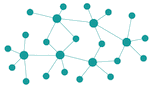
\includegraphics[scale=0.3]{./static/decentnew.png} & 
\includegraphics[scale=0.3]{./static/opensource.png} & 
\includegraphics[scale=0.3]{./static/privacy.png}\\ 
\textbf{Decentralized} & \textbf{Open source} & \textbf{Designed for privacy.png}\\
\hline
Infinitely Scalable, built using P2P architecture. Without single point of failure – no central company or server. & All source code is always visible, empowering contributions \& 100\% transparency. & Powerful encryption, Node Reputation, Layered Protection Protocols, etc.. All working to help you safely \& privately participate in the Network. \\
 \hline
\end{tabularx}
\end{adjustbox}

\end{frame}
 

\begin{frame}[t]{Evolution of internet \& crypto currencies}
 
\textbf{Netscape moment}: \emph{Cambrian} explosion of crypto-currency Ðapps
 
% \newcolumntype{Y}{>{\centering\arraybackslash}X}

 \begin{adjustbox}{width=.75\textwidth}
\begin{tabularx} {\textwidth}{|X|X|X|X|}
 \hline
& 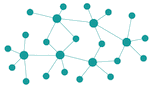
\includegraphics[scale=0.2]{static/decentnew} & 
\includegraphics[scale=0.2]{static/hootcoin} & \\
 \hline
\textbf{Phase} & \textbf{Internet} & \textbf{Crypto-currency} & \textbf{Reach}\\
\hline
Protocol & TCP/IP, SMTP & bitgold, \textbf{Bitcoin}, Ethereum & 1M People \\
\hline
Infrastructure & ISPs, lay fiber & \textbf{Exchanges}, secure storage & 10M people \\
\hline
Consumer Interface & Browser & User controlled \textbf{btc/eth wallets} & 100M people \\
\hline
Decentralized Ðapps & Web 2.0 & Finance 2.0 Ðapps & 1B people\\
\hline
Fat Protocols & Web 3.0 & Filecoin, \textbf{GPUCoin ICO} empower next-gen Ðapps & 2B people\\

\hline
\end{tabularx}
\end{adjustbox}

Protocol layer like \textbf{File}-coin and \textbf{GPU}-Coin ICO is the next Web 3.0 
\end{frame} 
 
 \begin{frame}[t]{IPCN: InterPlanetary Compute Network}
	%TeraFlop/PetaFlop super-computer grade
	
\includegraphics[scale=.3]{static/ipcn-p2p}
	 Uber/Airbnb for GPU computers
 \begin{itemize}
 \item Build \textbf{TeraFlop/PetaFlop super-computers} on top of the  Hoot GPUcoin \textbf{I}nter-\textbf{P}lanetary \textbf{C}ompute \textbf{N}etwork(IPCN)
 \item architecture revolving around fault tolerant redundant P2P, Blockchain, Smart Contracts, State Channels
 \item a platform to create new compute primitives using any Turing compute programming language
 \item use container technologies such as docker \& kubernetes to efficiently distribute \& use excess unused GPU compute
 \item powered by cryptocurrency micro-payments
 \item compute results verifiable using cryptographic \& mathematical properties
 \end{itemize}
\end{frame}
% \begin{frame}[t]{IPCN: Interplanetary Compute Network}
% 	
\includegraphics[scale=.3]{static/ipcn-p2p} Uber/Airbnb for computers
% \begin{itemize}
% \item architecture revolving around fault tolerant redundant P2P, Blockchain, Smart Contracts, State Channels
% \item a platform to create new compute primitives using any turing compute programming language
% \item use container technologies such as docker \& kubernetes to efficiently distribute \& use excess unused compute
% \item powered by cryptocurrency micro-payments
% \item compute results verifiable using cryptographic \& mathematical properties
% \end{itemize}
% \end{frame}

%--- Next Frame ---%
\begin{frame}[t]{GPUcoin GPC Tokens }
 

\includegraphics[scale=0.2]{static/hootcoin} Decentralized P2P	 GPUcoin GPC nodes will earn crypto-token incentives called GPUcoins GPC

 \begin{itemize}[<+-| alert@+>]
 \item for contributing their \textbf{GPU} processing power \& bandwidth in the service of mining, GPU compute, encoding \& distributing video using the GPUcoin live virtual-machine 
 \item for participating in the GPUcoin IPCN \textbf{I}nter\textbf{P}lanetary \textbf{C}ompute \textbf{N}etwork \& security protocol
 \item much like miners in Bitcoin \& Ethereum earn token for mining the \textbf{cryptocurrency} in exchange for \textbf{breaking complex math puzzles}
 \item GPUcoin tokens are \textbf{paid API keys i.e., utility tokens} \underline{NOT} securities you can redeem GPUcoin GPC  tokens for GPU compute time/bandwidth on the decentralized GPUcoin compute IPCN™\textsuperscript{TM}  network
 \end{itemize}
 
\end{frame}
%--- Next Frame ---%

\section{Conclusion}

\begin{frame}{Summary}


\includegraphics[scale=.4]{static/ipcn-p2p}
IPCN™\textsuperscript{TM} Get the GPUcoin GPC tokens from

\includegraphics[scale=0.4]{static/hootcoin} 
 \begin{center}\url{http://onhoot.com/tokensale}\end{center}



 % The theme \emph{itself} is licensed under a
 % \href{http://creativecommons.org/licenses/by-sa/4.0/}{Creative Commons
 % Attribution-ShareAlike 4.0 International License}.

 \begin{center}\ccbysa\end{center}

\end{frame}

\begin{frame}[standout]
 Questions?
\end{frame}


\end{document}


\section{Titleformats}

\begin{frame}{Metropolis titleformats}
	\themename supports 4 different titleformats:
	\begin{itemize}
		\item Regular
		\item \textsc{Smallcaps}
		\item \textsc{allsmallcaps}
		\item ALLCAPS
	\end{itemize}
	They can either be set at once for every title type or individually.
\end{frame}

{
 \metroset{titleformat frame=smallcaps}
\begin{frame}{Small caps}
	This frame uses the \texttt{smallcaps} titleformat.

	\begin{alertblock}{Potential Problems}
		Be aware, that not every font supports small caps. If for example you typeset your presentation with pdfTeX \& the Computer Modern Sans Serif font, every text in smallcaps will be typeset with the Computer Modern Serif font instead.
	\end{alertblock}
\end{frame}
}

{
\metroset{titleformat frame=allsmallcaps}
\begin{frame}{All small caps}
	This frame uses the \texttt{allsmallcaps} titleformat.

	\begin{alertblock}{Potential problems}
		As this titleformat also uses smallcaps you face the same problems as with the \texttt{smallcaps} titleformat. Additionally this format can cause some other problems. Please refer to the documentation if you consider using it.

		As a rule of thumb: Just use it for plaintext-only titles.
	\end{alertblock}
\end{frame}
}

{
\metroset{titleformat frame=allcaps}
\begin{frame}{All caps}
	This frame uses the \texttt{allcaps} titleformat.

	\begin{alertblock}{Potential Problems}
		This titleformat is not as problematic as the \texttt{allsmallcaps} format, but basically suffers from the same deficiencies. So please have a look at the documentation if you want to use it.
	\end{alertblock}
\end{frame}
}

\section{Elements}

\begin{frame}[fragile]{Typography}
 \begin{verbatim}The theme provides sensible defaults to
\emph{emphasize} text, \alert{accent} parts
or show \textbf{bold} results.\end{verbatim}

 \begin{center}becomes\end{center}

 The theme provides sensible defaults to \emph{emphasize} text,
 \alert{accent} parts or show \textbf{bold} results.
\end{frame}

\begin{frame}{Font feature test}
 \begin{itemize}
 \item Regular
 \item \textit{Italic}
 \item \textsc{SmallCaps}
 \item \textbf{Bold}
 \item \textbf{\textit{Bold Italic}}
 \item \textbf{\textsc{Bold SmallCaps}}
 \item \texttt{Monospace}
 \item \texttt{\textit{Monospace Italic}}
 \item \texttt{\textbf{Monospace Bold}}
 \item \texttt{\textbf{\textit{Monospace Bold Italic}}}
 \end{itemize}
\end{frame}

\begin{frame}{Lists}
 \begin{columns}[T,onlytextwidth]
 \column{0.33\textwidth}
 Items
 \begin{itemize}
 \item Milk \item Eggs \item Potatoes
 \end{itemize}

 \column{0.33\textwidth}
 Enumerations
 \begin{enumerate}
 \item First, \item Second \& \item Last.
 \end{enumerate}

 \column{0.33\textwidth}
 Descriptions
 \begin{description}
 \item[PowerPoint] Meeh. \item[Beamer] Yeeeha.
 \end{description}
 \end{columns}
\end{frame}
\begin{frame}{Animation}
 \begin{itemize}[<+- | alert@+>]
 \item \alert<4>{This is\only<4>{ really} important}
 \item Now this
 \item \& now this
 \end{itemize}
\end{frame}
\begin{frame}{Figures}
 \begin{figure}
 \newcounter{density}
 \setcounter{density}{20}
 \begin{tikzpicture}
 \def\couleur{alerted text.fg}
 \path[coordinate] (0,0) coordinate(A)
  ++( 90:5cm) coordinate(B)
  ++(0:5cm) coordinate(C)
  ++(-90:5cm) coordinate(D);
 \draw[fill=\couleur!\thedensity] (A) -- (B) -- (C) --(D) -- cycle;
 \foreach \x in {1,...,40}{%
 \pgfmathsetcounter{density}{\thedensity+20}
 \setcounter{density}{\thedensity}
 \path[coordinate] coordinate(X) at (A){};
 \path[coordinate] (A) -- (B) coordinate[pos=.10](A)
  -- (C) coordinate[pos=.10](B)
  -- (D) coordinate[pos=.10](C)
  -- (X) coordinate[pos=.10](D);
 \draw[fill=\couleur!\thedensity] (A)--(B)--(C)-- (D) -- cycle;
 }
 \end{tikzpicture}
 \caption{Rotated square from
 \href{http://www.texample.net/tikz/examples/rotated-polygons/}{texample.net}.}
 \end{figure}
\end{frame}
\begin{frame}{Tables}
 \begin{table}
 \caption{Largest cities in the world (source: Wikipedia)}
 \begin{tabular}{@{} lr @{}}
 \toprule
 City & Population\\
 \midrule
 Mexico City & 20,116,842\\
 Shanghai & 19,210,000\\
 Peking & 15,796,450\\
 Istanbul & 14,160,467\\
 \bottomrule
 \end{tabular}
 \end{table}
\end{frame}
\begin{frame}{Blocks}
 Three different block environments are pre-defined \& may be styled with an
 optional background color.

 \begin{columns}[T,onlytextwidth]
 \column{0.5\textwidth}
 \begin{block}{Default}
 Block content.
 \end{block}

 \begin{alertblock}{Alert}
 Block content.
 \end{alertblock}

 \begin{exampleblock}{Example}
 Block content.
 \end{exampleblock}

 \column{0.5\textwidth}

 \metroset{block=fill}

 \begin{block}{Default}
 Block content.
 \end{block}

 \begin{alertblock}{Alert}
 Block content.
 \end{alertblock}

 \begin{exampleblock}{Example}
 Block content.
 \end{exampleblock}

 \end{columns}
\end{frame}
\begin{frame}{Math}
 \begin{equation*}
 e = \lim_{n\to \infty} \left(1 + \frac{1}{n}\right)^n
 \end{equation*}
\end{frame}
\begin{frame}{Line plots}
 \begin{figure}
 \begin{tikzpicture}
 \begin{axis}[
 mlineplot,
 width=0.9\textwidth,
 height=6cm,
 ]

 \addplot {sin(deg(x))};
 \addplot+[samples=100] {sin(deg(2*x))};

 \end{axis}
 \end{tikzpicture}
 \end{figure}
\end{frame}
\begin{frame}{Bar charts}
 \begin{figure}
 \begin{tikzpicture}
 \begin{axis}[
 mbarplot,
 xlabel={Foo},
 ylabel={Bar},
 width=0.9\textwidth,
 height=6cm,
 ]

 \addplot plot coordinates {(1, 20) (2, 25) (3, 22.4) (4, 12.4)};
 \addplot plot coordinates {(1, 18) (2, 24) (3, 23.5) (4, 13.2)};
 \addplot plot coordinates {(1, 10) (2, 19) (3, 25) (4, 15.2)};

 \legend{lorem, ipsum, dolor}

 \end{axis}
 \end{tikzpicture}
 \end{figure}
\end{frame}
\begin{frame}{Quotes}
 \begin{quote}
 Veni, Vidi, Vici
 \end{quote}
\end{frame}

{%
\setbeamertemplate{frame footer}{My custom footer}
\begin{frame}[fragile]{Frame footer}
 \themename defines a custom beamer template to add a text to the footer. It can be set via
 \begin{verbatim}\setbeamertemplate{frame footer}{My custom footer}\end{verbatim}
\end{frame}
}

\begin{frame}{References}
 Some references to showcase [allowframebreaks] \cite{knuth92,ConcreteMath,Simpson,Er01,greenwade93}
\end{frame}

\section{Conclusion}

\begin{frame}{Summary}

 Get the source of this theme \& the demo presentation from

 \begin{center}\url{github.com/matze/mtheme}\end{center}

 The theme \emph{itself} is licensed under a
 \href{http://creativecommons.org/licenses/by-sa/4.0/}{Creative Commons
 Attribution-ShareAlike 4.0 International License}.

 \begin{center}\ccbysa\end{center}

\end{frame}

\begin{frame}[standout]
 Questions?
\end{frame}

\appendix
\begin{frame}[t]{Centralized vs Decentralized 
}
 % \begin{table}
 % \caption{Central vs P2P benefits (source: Crypto blockchain thesis)}

\begin{table}[ht]
\centering
\begin{adjustbox}{width=1\textwidth}

 \begin{tabularx}{\textwidth}{|Y|Y|}
 % \begin{tabular}{@{} |l|r| @{}}
 \toprule
 Facebook/Twitter & Hoot decentralized\\
 
\includegraphics[scale=0.25]{static/cent} & 
\includegraphics[scale=0.25]{static/dec}\\
 \midrule
 Focus on Shareholder benefit & Focus on Network participant benefits\\
 Your private data in everyone hands & Your Private data is Decentralized\\
 Simplified access to your data & Restricted access of your data \\
 High profit margins & Perfect competition sets fair price\\
 \textbf{Heavily censored} & \textbf{Censorship-free}\\
 Not fault tolerant & a dense Byzantine fault tolerant \\
 not peer to peer & peer-to-peer network\\
 \bottomrule
 \end{tabularx}
 \end{adjustbox}
 \end{table}
\end{frame}
\begin{frame}[fragile]{Backup slides}
 Sometimes, it is useful to add slides at the end of your presentation to
 refer to during audience questions.

 The best way to do this is to include the \verb|appendixnumberbeamer|
 package in your preamble \& call \verb|\appendix| before your backup slides.

 \themename will automatically turn off slide numbering \& progress bars for
 slides in the appendix.
\end{frame}

\begin{frame}[allowframebreaks]{References}

 \bibliography{demo}
 \bibliographystyle{abbrv}

\end{frame}

\end{document}
